\chapter{Javascript}

\section{The Basics}

Javascript heisst eigentlich ECMAScript, welches aktuell in Version 6 vorliegt. Browser unterstützen aber nur Version 5.1. Zudem gibt es noch eine \lstinline|strict|-Version der Sprache. Ist der \lstinline|strict|-Modus aktiviert, muss man z.B. alle Variablen mit \lstinline|var| deklarieren. Um den \lstinline|strict|-Modus zu aktivieren muss man \lstinline|"use strict";| als erste Anweisung des Skriptes oder einer Funktion schreiben. Best Practice: Verwende  \lstinline|strict|-Modus. 

In Javascript gibt es nur Objekte und keine Klassen. Listing \ref{lst:objekte-deklarieren} zeigt einige Code-Beispiele im Umgang mit Objekten.

\begin{lstlisting}[label=lst:objekte-deklarieren,caption=Objekte deklarieren]
// Objekt durch Object Literal definieren
var bachelorModule = {
	title: "WebApplication Development",
	print: function() { console.log(this.title) }
};
bachelorModule.title;
bachelorModule["title"]; // Als assoziatives Array
bachelorModule.print();

// Objekt durch Constructor (immer grossschreiben) deklarieren
function Name(vorname, nachname) {
	this.vorname = vorname;
	this.nachname = nachname;
}
Name.prototype.hello = function(){
	return "Hello" + this.vorname;
}

var name = new Name("Thomas", "Koller");
console.log(name.vorname);
console.log(name.hello());
// Property hinzufügen
name.age = 99;
// Property entfernen
delete name.age;
// nicht definiertes Property
console.log(name.age); // undefined
// nach Property testen
name.hasOwnProperty("vorname"); // true
// Getter / Setter ab ES5
var otherModule = {
	get title() {return "test"},
	set title(value) {}
};
console.log(otherModule.title); // So kann auf Getter zugegriffen werden
console.log(typeof a); //typeof-Operator
\end{lstlisting}

In JavaScript enthält jedes Objekt implizit ein Property dass auf einen Prototypen zeigt. Diese Prototypen sind verkettet, wobei das letzte Objekt der Kette auf den \lstinline|null|-Prototyp zeigt. Wird ein Property im Objekt selbst nicht gefunden, wird die Prototyp-Kette danach durchsucht. Mit Hilfe der Methode \lstinline|Object.getPrototypeOf()| (ES5) kann explizit auf den Prototype zugegriffen werden. Abbildung \ref{fig:prototyp} zeigt wie die Properties \lstinline|vorname| und \lstinline|nachname| beim jeweiligen Objekt sind und die Methode \lstinline|hello()| von beiden Objekten beim Prototyp nachgeschlagen. Der Prototyp selbst, zeigt auf den \lstinline|null|-Prototyp.

\begin{figure}
\centering
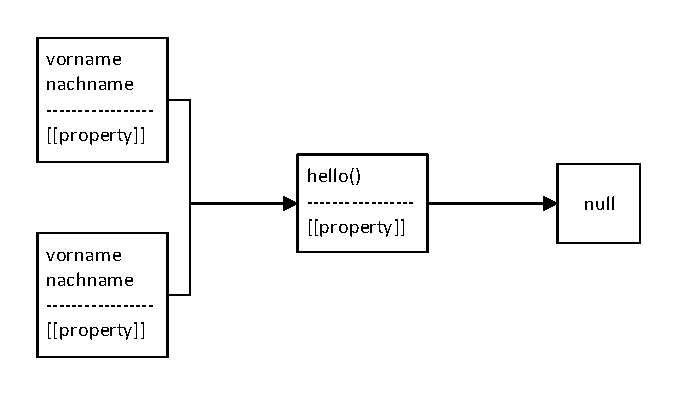
\includegraphics[width=0.7\linewidth]{fig/prototyp}
\caption{Prototyp}
\label{fig:prototyp}
\end{figure}

JavaScript unterstützt JSON von Haus aus. Listing \ref{lst:json} zeigt einige Beispiele zu JSON und Arrays.

\begin{lstlisting}[label=lst:json,caption=JSON]
// JSON.stringify ruft eine Methode toJSON auf (falls diese existiert) und 
// serialisiert das Objekt das zurückgegeben wird
otherModule.toJSON = function(key) {
	var other = {course: this.course, semester: this.semester};
	return other;
}
var otherBachelorModule = JSON.parse(JSON.stringify(otherModule));
console.log(otherBachelorModule);

// Deklaration von Arrays
// Array Literals
var empty = [];
var full = [1,3,8];
var mixed = ["yes", true, 1, 5.0];
var objectArray = [{a:1, b:2}, {a:7,c:15}];

// Array mit new
var another = new Array(); // empty
var oneMore = new Array(5);

// Array Zugriff und Elemente hinzufuegen
var a = ["one"];
console.log(a[0]); // one
a[1] = "two";
console.log(a.length); // 2

// sparse Array
a[1000] = "thousand"; // Tausendstes Element ist besetzt der Rest ist leer
console.log(a[500]); // undefined

// for loop for sparse arrays
for (var index in a) {
	console.log(a[index]); // one, two, thousand
}

// Weitere Array Methoden -> Buch
// Beispiel reduce (ES5)
var a = [1,2,3,4,5,6];
var sum = a.reduce(function(x,y) {return x+y;}, 0);
console.log(sum); // 21
\end{lstlisting}

In JavaScript sind Funktionen ebenfalls Objekte. Sie erhalten als unsichtbaren Parameter das Keyword \lstinline|this|. Der Wert von \lstinline|this| ist davon abhängig wie die Funktion aufgerufen wird. Listing \ref{lst:methoden-aufruf} zeigt wie Funktionen deklariert und aufgerufen werden. Es gibt vier Möglichkeiten eine Funktion aufzurufen (Invocation Patterns).

\begin{lstlisting}[label=lst:methoden-aufruf,caption=Methoden aufrufen]
// Anonyme Funktion erstellen und an Variable binden
var add = function(a,b) { return a+b; }

// Funktion mit Name an Variable binden (wenn man Funktion rekursiv aufrufen will)
var sub = function sub(a,b) { return a-b; }

// Funktion mit Name ohne an Variable zu binden
function mult(a,b) { return a*b; }

// 1. Funktion mit Name aufrufen
mult(4,5);

// 2. Funktion sofort aufrufen
var fiveToThePowerOfTwo = function(x){return x*x;}(5);
console.log(fiveToThePowerOfTwo); // 25

// 3. Funktion als Literal aufrufen
var aPerson = {
	preName: "Thomas",
	name: "Koller",
	getFullName: function () {
		return this.preName + " " + this.name;
	}
};
console.log(aPerson.getFullName());

// 4. Funktion von anderem Objekt mit apply aufrufen
var dDuck = {
	preName: "Donald",
	name: "Duck"
}

dDuck.getFullName(); // undefined

var donaldsName = aPerson.getFullName.apply(dDuck);
console.log(donaldsName); // Donald Duck
\end{lstlisting}

In Javascript wird nur pro Funktion ein neuer Scope erstellt. In Listing \ref{lst:scope} werden zwei For-Schlaufen erstellt welche zwei Variablen deklarieren. Eigentlich ist es aber nur eine Variable, weil alle Variablendeklarationen an den Anfang einer Funktion gezogen werden (Hoisting).

\newpage

\begin{lstlisting}[label=lst:scope,caption=Scope]
function scopeTest() {
	for(var i = 0; i < 10; i++) {
		console.log(i);
	}
	for(var i = 0; i < 10; i++) {
		console.log(i);
	}
}
// Javascript zieht Variable an den Funktionsanfang (Hoisting)
function scopeTest() {
	var i;
	for(i = 0; i < 10; i++) {
		console.log(i);
	}
	for(i = 0; i < 10; i++) {
		console.log(i);
	}
}
\end{lstlisting}

In JavaScript haben Funktionen Zugriff zum äusseren Scope. Weil auch jede Funktion ein Objekt ist, ist es möglich Closures zu erstellen. Ein Closure kann auch zu einem späteren Zeitpunkt auf seine äusseren Variablen zugreifen, auch wenn dieser Code schon abgearbeitet wurde. Dadurch lassen sich z.B. private Eigenschaften für Objekte erstellen, wie Listing \ref{lst:closure} zeigt.

\begin{lstlisting}[label=lst:closure,caption=Closure]
var myCounter = (function () {
	var value = 0;
	return {
		increment: function (inc) {
			value += inc;
		},
		getValue: function () {
			return value;
		}
	};
}()); // Funktion wird sofort aufgerufen

myCounter.increment(10);
console.log(myCounter.getValue()); // 10
console.log(myCounter.value); // undefined
\end{lstlisting}

Ein Vorteil von Java ist die Objektorientierung und auch die literale Syntax um Objekte zu erstellen. Auch Closures kann man ohne Probleme verwenden. Man sollte darauf achten dass man immer mit \lstinline|===| und nicht mit \lstinline|==|, sonst werden die Werte komisch umgewandelt. Auch die Verwendung von Prototypen und \lstinline|with| sollte man vermeiden. Besondere Vorsicht ist bei globalen Variablen, dem Scope und den Einfügeregeln von Semikolons geboten. Auch das Schlüsselwort \lstinline|typeof| und \lstinline|eval| sind nicht zuverlässig.

\newpage

\subsection{Javascript einbinden}
Javascript kann über vier Wege eingebunden werden:
\begin{description}
	\item[Inline] Innerhalb des HTML-Tag \lstinline|<script></script>| kann direkt Javascript-Code geschrieben werden.
	\item[External File] Javascript-Code kann in externe Dateien ausgelagert werden, dafür wird folgendes HTML-Tag mit dem Attribut \lstinline|src| benötigt: \lstinline|<script src="something.js"/>|. Der Vorteil der Auslagerung besteht darin, dass Verhalten und Struktur komplett separiert sind und die Wiederverwendung des Javascript-Codes erhöht wird. Ausserdem können die Dateien gecached werden.
	\item[HTML event handler] Beliebiges Javascript kann in spezifischen Attribute in HTML eingefügt werden: \lstinline|<input type="checkbox" name="options" value="giftwrap" onchange="order.options.giftwrap = this.checked;">|. Oft werden einfach Funktionen aufgerufen.
	\item[URL mit javascript: protocol] Wie beispielsweise: \lstinline|<a href="javascript:void(0)">login</a>|.
\end{description}

Die Verarbeitung von Javascript läuft in zwei Phasen ab: In der ersten Phase wird Inline-Javascript ausgeführt und die externen Javascript Files geladen, welche synchron (default), asynchron (\lstinline|<script async>|) oder defered (\lstinline|<script defer>|) ausgeführt werden. Bei async wird der Javascript parallel zum HTML Parsing heruntergeladen und nach dem Download direkt ausgeführt. Bei defer wird der Code auch parallel zum HTML Parsing heruntergeladen aber erst nach dem HTML Parsing ausgeführt\footnote{\url{http://www.growingwiththeweb.com/2014/02/async-vs-defer-attributes.html}}. In der zweiten Phase werden die Event Handler asynchron ausgeführt. 

\subsection{Timeout und Interval}
\begin{lstlisting}[label=lst:timeout-interval,caption=Timeout \& Interval]
// Die Funktion f wird nach repetitiv nach Ablauf der Zeit interval mit den Argumenten args ausgeführt.
long setInterval(function f, unsigned long interval, any args...)

// Die Funktion f wird nach Ablauf der Zeit timeout genau einmal mit den Argumenten args ausgeführt.
long setTimeout(function f, unsigned long timeout, any args...)

function myFunction() { alert("Hey!"); }

myTimeout = setTimeout(myFunction, 3000);
clearTimeout(myTimeout);

myInterval = setInterval(myFunction, 1000);
clearInterval(myInterval);
\end{lstlisting}

\newpage

\subsection{DOM und CSS Manipulation}
Mit Javascript wird primär der DOM manipuliert. 

\begin{lstlisting}[label=lst:dom-manipulation,caption=DOM Manipulation]
// Selektion über ID, ID sollte immer indeutig sein
var elt = document.getElementById("quack");

// Selektion über nicht eindeutigen Name, kann auch mehrere Elemente zurückgeben
var radiobuttons = document.getElementsByName("favorite_color");

// Selektion über Tag-Name
var firstpara = document.getElementsByTagName("p")[0];
var firstParaSpans = firstpara.getElementsByTagName("span");

// Selektion über CSS-Klasse
var warnings = document.getElementsByClassName("warning");

// Selektion über CSS-Selektoren (HTML5 spezifisch - kennen wir aus jQuery)
var logs = document.querySelectorAll("#log>span");

// DOM-Elemente erzeugen
createElement()
createTextNode()
createComment()
createDocumentFragment() // Hier können vorab grosse Strukturen erstellt werden und auf einen Schlag im Browser dargestellt werden, der Benutzer bekommt nichts mit.

appendChild()
insertBefore()
removeChild()
replaceChild()

// CSS Manipulation
e.style.fontSize = "12pt";
e.style.font-size = "12pt"; // Achtung: Geht nicht!

// Event-Handlers
window.onload = function() {...}
// folgendes ist Equivalent, aber als "schöner" betitelt.
window.addEventListener("load", function(){...});

// Ajax
var request = new XMLHttpRequest();
request.open("GET", "http://test.ch/data.json");
request.setRequestHeader("Content-Type", "text/plain");
request.send();
request.onreadystatechange = function() {
	if (request.readyState === 4 && request.status === 200) {
		var type = request.getResponseHeader("Content-Type");
		if (type.match(/^text/)) {
			// do something with request.responseText()
		}
	}
}
\end{lstlisting}

\newpage

Wir wissen, dass die HTML Struktur in-Memory als DOM repräsentiert wird. Wir können auf die einzelnen Nodes über folgende Attribute zugreifen: parentNode, childNodes, firstChild, lastChild, nextSibling, previousSibling, nodeType, nodeValue, nodeName. Als Beispiel \lstinline|document.childNodes[0].childNodes[1];|. HTML Attribute können wir über Javascript-Properties abfragen: \lstinline|var imgurl = image.src;|. Für alle Nicht-HTML Attribute kann setAttribute, getAttribute, hasAttribute und removeAttribute verwendet werden.

Den Inhalt von Elementen kann auf drei Sichtweisen betrachtet werden. Als Beispiel dient \lstinline|<p>This is a <i>simple</i> document.</p>|:
\begin{description}
	\item[HTML-String:] \textit{<p>This is a <i>simple</i> document.</p>}
	\item[Plain-Text:] \textit{This is a simple document.}
	\item[Node-Struktur:] Nodes im DOM
\end{description}
InnerHTML ist Content innerhalb des HTML Element und OuterHTML bedeutet den Inhalt des Element sowie das Element selber.

\section{Typescript}

\subsection{Javascript Issues}
Typescript existiert nur, weil in Javascript Unzulänglichkeiten existieren. In Javascript kennen wir nur Objekte und keine Klassen. Es ist kein modulare Aufbau mittels Imports möglich. Die gesamte Sprache ist dynamisch typisiert. Die Unterscheidung zwischen undefinied und null ist merkwürdig. Zudem werden auch Syntax-Fehler nicht abschliessend validiert, da es eine interpretierende Sprache ist.

\subsection{Types}
Typescript hat fast die selben Typen wie Javascript. Zusätzlich kommt noch das Enum, Any und Void hinzu. Das Enum und Void verhalten sich gleich wie in Java. Der Datentyp Any steht für irgendeinen Typ. Man kann Any z.B. verwenden wenn man Benutzereingaben erhält oder Werte von 3rd party libraries. Zudem dient Any der Rückwärtskompatibilität zu normalem Javascript. Der Typ kann natürlich auch weggelassen werden. Listing \ref{lst:typescript-types} zeigt einige Codebeispiele.

\begin{lstlisting}[label=lst:typescript-types,caption=Types]
// Nachfolgende Typen sind gleich wie in Javascript
var isDone: boolean = false;
var height: number = 6; // In Typescript gibts auch nur Floating Points Numbers
var name: string = "bob" // Es können Single oder Double Quotes verwendet werden
var list:number[] = [1, 2, 3]; // Ein typisierter Array

// Nachfolgende Typen gibt es in JavaScript nicht
enum Color {Red, Green, Blue};
var c: Color = Color.Green;

var notSure: any = 4;
notSure = "maybe a string instead";
notSure = false; // okay, definitely a boolean

function warnUser(): void {
	alert("This is my warning message");
}
\end{lstlisting}

\subsection{Ambient Declarations}

Damit Typescript problemlos mit herkömmlichem Javascript verwendet werden kann, muss man dem Compiler von Typescript mitteilen, welche Variablen global zur Verfügung stehen. Dieser Mechanismus wird Ambient Declarations genannt. Die Deklarationen für 3rd party libraries werden in einem separaten \lstinline|*.d.ts| abgelegt. Verwendet man beispielsweise die globale \lstinline|process|-Variable von NodeJS, ohne sie vorher zu deklarieren, wird der Compiler eine Fehlermeldung ausspucken. Fügt man aber folgende Anweisung \lstinline|declare var process:any;| ein, lässt sich die Variable verwenden, ohne dass der Compiler reklamiert. Es lassen sich sogar Interfaces von Javascript-Libraries deklarieren. Diese Deklarationen sollte man allerdings mit Vorsicht geniessen, weil man dem Compiler ein Versprechen abgibt, dass diese Variable zur Laufzeit vorhanden ist. Ist sie nicht vorhanden, kann es zu einem Fehler kommen.

\subsection{Functions mit Types und optionalen/default Parametern}

In Typescript lassen sich wie in Javascript benannte oder anonyme Funktionen erstellen. Zusätzlich lassen sich aber die Parameter und der Rückgabewert mit einem Typ versehen. Wenn eine Funktion einer Variable zugewiesen wird, kriegt diese Variable der Typ dieser Funktion. Der Typ einer Funktion setzt sich aus den Typen der Parameter und des Rückgabewerts zusammen. In Typescript ist zudem jeder Funktionsparameter erforderlich. In Javascript hingegen ist jeder Parameter optional. Möchte man optionale Parameter in Typescript haben, muss man diese mit einem Fragezeichen markieren. Zudem kommen die optionalen Parameter immer nach den erforderlichen Parametern. Zudem können auch Default-Parameter mit einem Wert vordefiniert werden. Listing \ref{lst:typescript-functions} zeigt einige Codebeispiele.

\begin{lstlisting}[label=lst:typescript-functions,caption=Functions]
// Variable hat den Typ (x:number, y:number)=>number
var myAdd: (x:number, y:number)=>number = function(x: number, y: number): number { 
	return x+y; 
};

// Optionale Parameter
function buildName(firstName: string, lastName?: string) {}

// Default Parameter
function buildName(firstName: string, lastName = "Smith") {}
\end{lstlisting}

\subsection{Interfaces}

Interfaces in Typescript basieren auf dem \textit{duck typing} Prinzip. Das heisst ein Objekt muss nicht unbedingt \lstinline|implements| verwenden und es muss mindestens die Eigenschaften haben, die vom Interface vorgegeben werden. Das Objekt kann aber auch zusätzliche Eigenschaften haben als das Interface und der Code kompiliert trotzdem. Es ist zudem möglich optionale Attribute bei einem Interface zu deklarieren.

\begin{lstlisting}[label=lst:typescript-interfaces,caption=Interfaces]
interface LabelledValue {
	label: string;
	text?: string; // Optionales Attribute
}

// Funktion welche ein LablledValue nimmt
function printLabel(labelledObj: LabelledValue) {
	console.log(labelledObj.label);
}

// Das Objekt verwendet kein implements hat aber die Eigentschaft label und erfüllt 
// somit das Interface
let myObj = {size: 10, label: "Size 10 Object"};
printLabel(myObj);


interface ClockInterface {
	currentTime: Date;
	setTime(d: Date); // Methode auf Interface definiert
}

// Klasse implementiert Interface
class Clock implements ClockInterface {
	currentTime: Date;
	setTime(d: Date) {
		this.currentTime = d;
	}
	constructor(h: number, m: number) { }
}
\end{lstlisting}

\subsection{Classes}

Klassen in Typescript verhalten sich gleich wie in Java. Es gibt sogar abstrakte Klassen. Allerdings sind alle Instanzvariablen standardmässig \lstinline|public|. Zudem gibt es noch \lstinline|private| und \lstinline|protected|, welche sich auch wie in Java verhalten.

\begin{lstlisting}[label=lst:typescript-classes,caption=Classes]
class Animal {
	name: string;
	constructor(theName: string) { this.name = theName; }
	move(distanceInMeters: number = 0) {
		console.log(`${this.name} moved ${distanceInMeters}m.`);
	}
}

class Snake extends Animal {
	constructor(name: string) { super(name); }
	move(distanceInMeters = 5) {
		console.log("Slithering...");
		super.move(distanceInMeters);
	}
}

class Horse extends Animal {
	constructor(name: string) { super(name); }
	move(distanceInMeters = 45) {
		console.log("Galloping...");
		super.move(distanceInMeters);
	}
}

let sam = new Snake("Sammy the Python");
let tom: Animal = new Horse("Tommy the Palomino");

sam.move();
tom.move(34);
\end{lstlisting}

\newpage

\subsection{Modules}

In Typescript gibt es ein Modulsystem. Variablen, Funktionen usw. in einem Modul sind nicht mehr global sichtbar, ausser die welche explizit mit \lstinline|export| öffentlich gemacht wurden. Möchte man etwas von einem anderen Modul konsumieren muss man es mit dem \lstinline|import| in den eigenen Code einbinden. Jede Datei welche ein \lstinline|export| oder \lstinline|import| beinhaltet wird als Modul deklariert. 

\begin{lstlisting}[label=lst:typescript-modules,caption=Modules]
export const numberRegexp = /^[0-9]+$/;

export class ZipCodeValidator {
	isAcceptable(s: string) {
		return s.length === 5 && numberRegexp.test(s);
	}
}

import { ZipCodeValidator } from "./ZipCodeValidator";

let myValidator = new ZipCodeValidator();
\end{lstlisting}

\subsection{Alternativen}
Neben TypeScript ist in letzter Zeit auch CoffeeScript ziemlich populär geworden. Das Google Web Toolkit (GWT) ist mittlerweile auf dem sinkenden Ast (Java->Javascript).

\section{Libraries und Werkzeuge}

\subsection{Java Script Libraries für DOM-Manipulation}
\begin{itemize}
	\item jQuery: Absoluter König.
	\item YUI: Mittlerweile gestorben.
	\item mootools: Verhasst von Markus Ineichen.
	\item dojo toolkit
\end{itemize}

\subsection{Java Script Libraries für CSS}
\begin{itemize}
	\item bootstrap: Einfach und beliebt. CSS/Javascript Framework. Verinnerlicht den mobile first Ansatz, cooles Grid System.
	\item modernizr: Macht alte Browser modern!
	\item Kendo UI
	\item HTML5 Boilerplate: Gutes Template für eine HTML5 Seite. Beinhaltet HTML Template, Normalize.css, jQuery, Modernizer, Analytics u.v.m. Alternativ kann man sein Projekt auch mit yeoman aufsetzen.
\end{itemize}

\newpage

\subsection{Java Script Libraries für UI}
Das Javascript erzeugt eigentlich die Seite und wird nicht vom Server aufbereitet.
\begin{itemize}
	\item jQuery UI
	\item Angular JS
	\item Sencha
	\item ext js
	\item kendo ui
\end{itemize}

\subsection{Java Script Libraries für Build and Managing}
Folgende Tools stehen im Javascript Umfeld zur Verfügung.
\begin{description}
	\item[Grunt:] Task-Runner.
	\item[Gulp:] Task-Runner als Alternative zu Grunt - einfachere Konfiguration.
	\item[require js:] Definieren von Modulen und Abhängigkeiten zu anderen Modulen.
	\item[yeoman:] Erstellt das Gerüst von neuen Web Applikationen (scaffolding).
	\item[bower:] Package Manager für \textit{Front-End Assets} für den Browser - JavaScript, HTML, CSS etc. 
	\item[jslint:] Starke Syntax-Prüfung.
	\item[jshint:] Nachfolger von jslint, nicht mehr so stark. Wird nun eher präferiert.
\end{description}
Die Task-Runner sind vergleichbar mit ANT. Ich konfiguriere Tasks, welche beispielsweise Typescript zu Javascript kompilieren. Oder für folgendes: Linting, Testing, Concatenation,
Minification, Deployment. Linter prüfen Syntax und mögliche Fehler in Javascript.

\subsection{Qual der Wahl!}
Der Need definiert den Einsatz der jeweiligen Bibliothek. Im Web-Umfeld gibt es im Wochen-Zyklus neue Frameworks. Daher muss man Vorsicht walten lassen. Auf aktuelle aber bewährte Frameworks setzen!

Zudem kämpfen wir leider auch heute noch mit den Browser-Inkompatibilitäten. Wobei es langsam aber sicher immer besser wird. IE 6 ist nun endgültig vom Tisch. Auch IE 7 hat noch 1 Prozent Marktanteil.

\subsection{jQuery}
JQuery hilft uns im Bezug zu den Browser-Inkompatibilitäten. Es abstrahiert den Browser mit dem umständlichen und verbosen W3C DOM API. Wir können den DOM manipulieren, CSS anpassen, auf Browser-Events reagieren und AJAX-Requests absetzen. Wir können die Produktivität steigern, jedoch hat es keinen OO-Approach. Es gibt unterschiedliche Libraries:

\begin{itemize}
\item jQuery: Browser Facade
\item jQuery UI: User Interface Komponenten
\item jQuery Mobile: mobile UI Framework
\item QUnit: unit/component Testing Framework
\item Sizzle: CSS Selektoren (leichtgewichtiger)	
\end{itemize}

\begin{lstlisting}[label=lst:jquery-samples,caption=jQuery]
// In jQuery kann man alles aneinanderketten (chanining)
$("p.details").css("background-color", "yellow").show("fast");

// Es gibt 4 Anwendungen um jQuery aufzurufen:
// 1. Selektion
$(selector, context (optional)); 
// 2. Wrapper
$(document); $(window);
// 3. Erzeugen von HTML Elementen
var img = $("<img>", {src: url, css: {...}});
// 4. Onload
jQuery(function() {
	\\ jQuery code
});

// Getters/Setters
$("form").attr("action");
$("#icon").attr("src", "icon.gif");
$("#banner").attr({
	src: "banner.gif",
	alt: "Advertisement",
	width: 720, height: 64
});
$("a").attr("target", "_blank");

// CSS
$("h1").css("font-weight");
$("h1").css("fontWeight");
$("h1").css("font"); // Error: Compound style!
$("h1").css("font-variant", "smallcaps");
$("div.note").css("border", "solid black 2px");
$("h1").css({
	backgroundColor: "black",
	border: "dotted black 4px"
});

// Adding CSS classes
$("h1").addClass("hilite"); // Add a class
$("h1+p").addClass("hilite first"); // Add 2 classes

// Removing CSS classes
$("p").removeClass("hilite"); // Remove a class
$("p").removeClass("hilite first"); // Multiple classes
$("div").removeClass(); // Remove all classes

// Toggling CSS classes
$("tr:odd").toggleClass("oddrow"); // Adds or remove the class
$("p").hasClass("first") // Does any p element have this class?
$("#lead").is(".first") // This does the same thing
$("#lead").is(".first.hilite") // is() is more flexible than hasClass()

// Content
var title = $("head title").text() // Get document title
var headline = $("h1").html() // Get html of first <h1> element
$("h1").text(function(n,current) { // Give each heading a selection number
	return (n+1) + ": " + current
});

// Event Handlers
$("p").click(function() { $(this).css("background-color", "gray"); });

blur() focusin() mousedown() mouseup()
change() focusout() mouseenter() resize()
click() keydown() mouseleave() scroll()
dblclick() keypress() mousemove() select()
error() keyup() mouseout() submit()
focus() load() mouseover() unload()

// jQuery verwendet ein eigenes Event Objekt, das jedem Event Handler mitgegeben wird und Details über den Event enthält. Properties von "nativen" Event Objekten werden kopiert und ergänzt.

// jQuery Animationen
$("img").animate({ height: 0 });

fadeIn() fadeOut() fadeTo()
show() hide() toggle()
slideDown() slideUp() slideToggle()
animate()

// Ajax
setInterval(function() { $("#stats").load("status_report.html"); },60000);

// Load external script - Dynamically load a script from some other server
jQuery.getScript("http://example.com/js/widget.js");

// Load external script - Load a library and use it once it loads
jQuery.getScript("js/jquery.my_plugin.js", function() {
	$('div').my_plugin(); // Use the library we loaded
});

// JSON
jQuery.getJSON("data.json", function(data) {
	// data enthält das Objekt aus data.json
});

// Ajax
jQuery.ajax({
	type: "GET", // The HTTP request method.
	url: url, // The URL of the data to fetch.
	data: null, // Don't add any data to the URL.
	dataType: "script", // Execute the response as a script once we get it.
	success: callback // Call this function when done.
});

\end{lstlisting}

\newpage

\subsection{Beispiel Snippets}

\begin{lstlisting}[label=lst:sample-requirejs,caption=sample require.js]
requirejs.config({
	baseUrl: "scripts",
	paths: {
		jquery: '../bower_components/jquery/dist/jquery'
	}
});

require(['jquery', 'Go', 'GoBoardView', 'GoBoardModel', function ($, Go, GoBoardView, GoBoardModel, GoGameControl) {
	define('GoBoardModel', ['Go'], function(Go) {
		"use strict";
	/**
	* Create a new (empty) go board.
	* @param size the size of the go board
	* @constructor
	*/
	function GoBoardModel(size) {
	this.size = size;
	this.init();
}
\end{lstlisting}

\begin{lstlisting}[label=lst:sample-grunt,caption=sample Gruntfile]
module.exports = function(grunt) {
	grunt.initConfig({
		jshint: {
			files: ['Gruntfile.js', 'src/**/*.js', 'test/**/*.js'],
			options: {
				globals: {
					jQuery: true
				}
			}
		},
		watch: {
			files: ['<%= jshint.files %>'],
			tasks: ['jshint']
		}
	});

	grunt.loadNpmTasks('grunt-contrib-jshint');
	grunt.loadNpmTasks('grunt-contrib-watch');
	grunt.registerTask('default', ['jshint']);
};
\end{lstlisting}

\newpage

\begin{lstlisting}[label=lst:sample-gulp,caption=sample gulp]
// Include gulp
var gulp = require('gulp');

// Include Our Plugins
var jshint = require('gulp-jshint');
var sass = require('gulp-sass');
var concat = require('gulp-concat');
var uglify = require('gulp-uglify');
var rename = require('gulp-rename');

// Lint Task
gulp.task('lint', function() {
	return gulp.src('js/*.js')
	.pipe(jshint())
	.pipe(jshint.reporter('default'));
});

// Compile Our Sass
gulp.task('sass', function() {
	return gulp.src('scss/*.scss')
	.pipe(sass())
	.pipe(gulp.dest('dist/css'));
});
\end{lstlisting}

\section{Single Page Applications}

\subsection{Evolution}

Zu Beginn (1990) des Webs wurden nur statische HTML-Seiten ausgeliefert und diese im Browser gerendert. Als nächsten Schritt konnte auf dem Server dynamisch HTML erzeugt werden (z.B. mit PHP), es wurde aber immer noch alles auf dem Server verarbeitet. Ab 2005 kam mit Ajax und Javascript die Wende, welche die Benutzerfreundlichkeit deutlich steigerte. Zuerst wurde HTML per Ajax-Request vom Server abgefragt und mit Javascript im Browser ersetzt. Als letzten Entwicklungsschritt ab 2010 werden JSON-Daten per Ajax vom Server geholt und im Browser wird daraus das komplette HTML generiert. 

Damit hat sich das Rendering der Inhalte im Laufe der Zeit vom Server hin zum Client verschoben. Durch diese Evolution konnte der Browser das Betriebssystem abstrahieren, weil jedes Betriebssystem einen Browser hat und sich dieser mehr oder weniger überall gleich verhält. Dadurch entstehen immer mehr browserbasierte Programme (z.B. Office 365), wobei Gmail 2004 den Anfang machte.

Nachfolgend noch eine Gegenüberstellung von Web- zu Desktopapplikationen.

\begin{tabbing}
	\hspace{6cm}\=\kill
	\textbf{Web (SaaS)} \> \textbf{Desktop} \\
	\> \\
	Kein Backup nötig \> Security \\
	Kein Update \> Daten Hoheit \\
	Geringe Investitionskosten \> Hardware Zugriff \\
	Tiefe Setupkosten \> Features des Betriebssystem \\
	Pay as you Go \> Kalibrierte Systeme \\
\end{tabbing} 

\subsection{Definition}

Nachfolgend die Definition für SPA:
\begin{quote}
	Web app that fits on a single web page
	providing a fluid UX by loading all necessary
	code with a single page load
\end{quote}
Aus dieser Definition lassen sich folgende Charakteristiken ableiten:
\begin{itemize}
	\item Rich Client Applikation im Browser
	\item Reines HTML5 und JavaScript (kein Plugin)
	\item Kein erneuter Page reload
	\item  Die URL ändert nur hinter \# (oder wie gewohnt)
	\item Back-Button funktioniert
	\item Links sind Bookmark-bar
	\item Funktionalität offline zu gehen
	\item Harmoniert perfekt mit Restful Web Services
\end{itemize}
Abgeleitet von den oben genannten Charakteristiken ergeben sich folgende Vorteile:
\begin{itemize}
	\item Reach (Läuft auf jeder Plattform)
	\item Rich User Experience
	\item Reduced Round Tripping
\end{itemize}

\subsection{Komponenten}

Abbildung \ref{fig:spa-komponenten} zeigt den Aufbau einer typischen SPA.

\begin{figure}[h!]
\centering
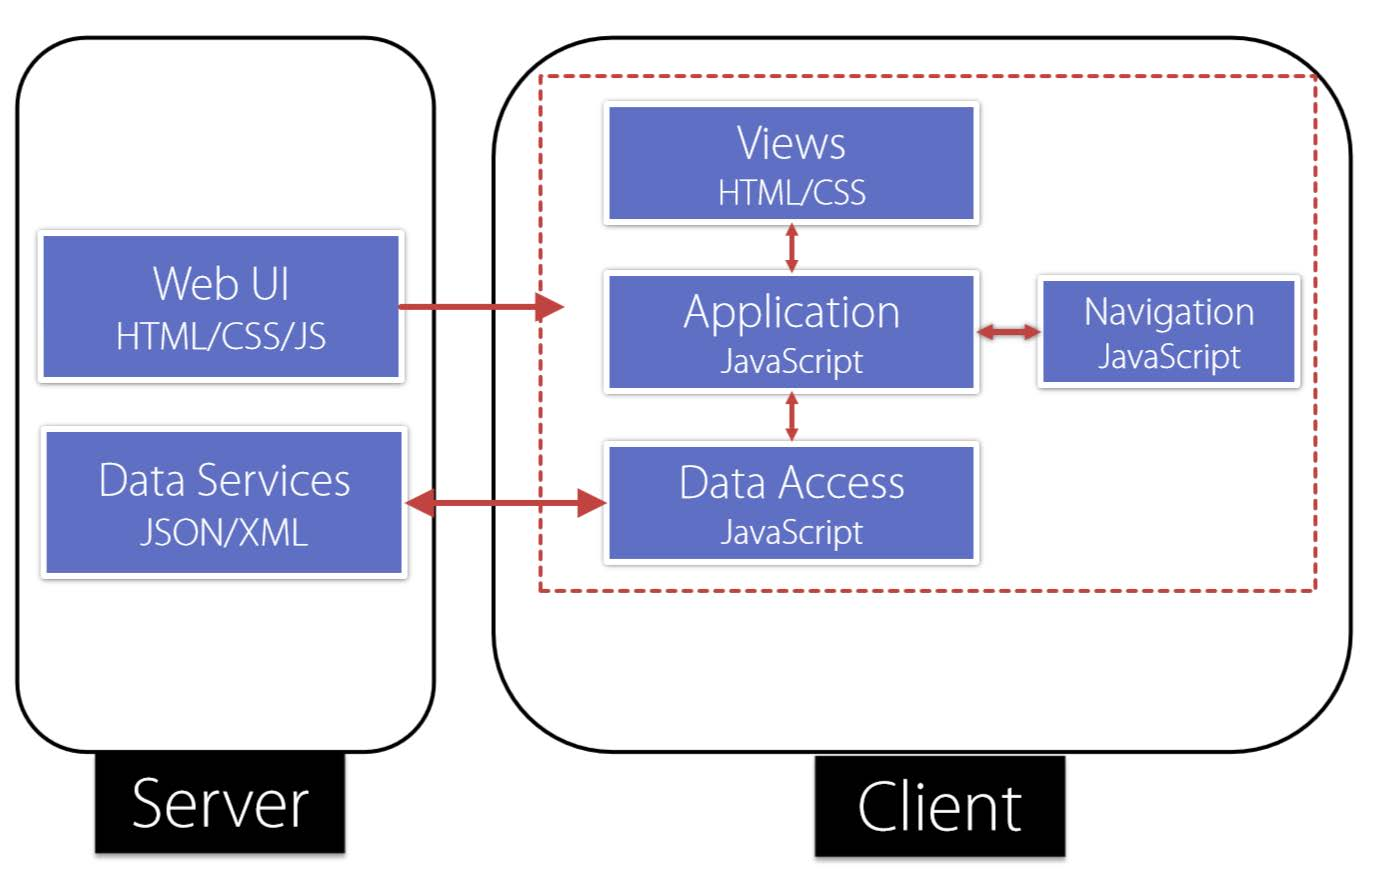
\includegraphics[width=0.7\linewidth]{fig/spa-komponenten}
\caption{SPA Komponenten}
\label{fig:spa-komponenten}
\end{figure}

\newpage

Demzufolge besteht eine SPA aus folgenden Komponenten:
\begin{description}
	\item[Routing (Navigation)] \hfil \\
	Das clientseitige Routing ermöglicht eine Navigation auf der Seite ohne Page Reload. Zudem muss der Backbutton und die Browserhistory (inkl. Bookmarks) wie gewohnt funktionieren. Vor HTML 5 wurde das mit einem Anchor (z.B. \lstinline|/#/home|) gelöst. HTML 5 bietet dafür eine eigene API mit der sich auch die Browserhistory ansteuern lässt.
	\item[Template-Rendering (View)] \hfil \\
	Beim Template-Rendering werden das Model über den Controller mit der View (HTML) verknüpft. Durch die Entkopplung der UI wird eine bessere Testbarkeit garantiert und durch das Binding reduziert sich der Code für das Updaten der Daten in der View.
	\item[(Remote-)Daten Zugriff] \hfil \\
	Die Daten werden meisten über eine REST-Schnittstelle bezogen und können bei Bedarf Zwischengespeichert werden (Cache). Die REST-Schnittstelle wird mit einem XHR-Request angesteuert und für den Cache lässt sich der LocalStorage auf dem Client verwenden.
	\item[Modularisierung des Codes] \hfil \\
	Durch die Modularisierung des Codes ergibt sich eine klare Struktur und was zu einer besseren Wart- bzw. Testbarkeit führt. Es sind zahlreiche Frameworks vorhanden die ein Modulsystem mitbringen (z.B. RequireJS oder TypeScript).
\end{description}

\section{Angular 2}

Angular 2 ist die zweite Version des SPA Frameworks für CRUD Anwendungen. Mit dem Framework muss man weniger Boilerplate Code schreiben und man kann seine Applikation sauber in Komponenten unterteilen. Es bietet Dependency Injection, ein performantes Binding an die View und die Unterteilung des UIs in Komponenten. Angular 2 setzt voll auf Typescript. Abbildung \ref{fig:angular2-architecture} gibt einen Überblick über die Architektur von Angular 2.
\begin{figure}[h!]
\centering
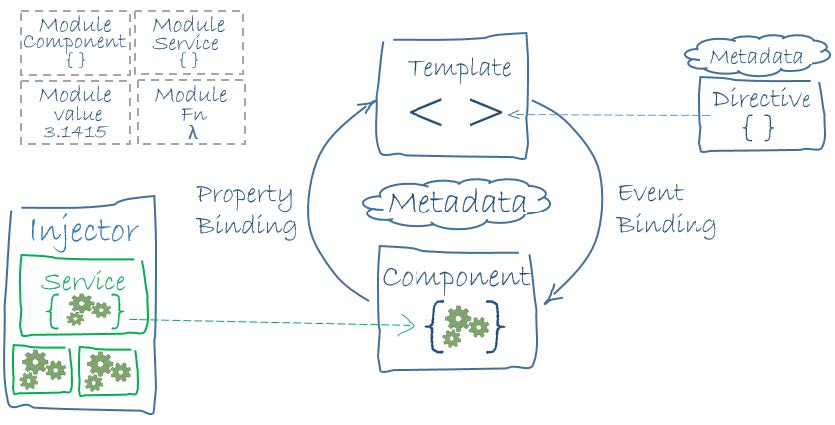
\includegraphics[width=0.7\linewidth]{fig/angular2-architecture}
\caption{Angular 2 Architektur Übersicht}
\label{fig:angular2-architecture}
\end{figure}

\newpage

Daraus lassen sich folgende Elemente erkennen:
\begin{description}
	\item[Module] \hfil \\
	Eine Angular App sollte aus Modulen bestehen, die gewisse Dinge (Klassen, Funktionen, Werte usw.) exportieren und von anderen Modulen importiert werden können. Sie lassen sich mit den Packages aus Java oder mit Namespaces aus .NET vergleichen. Das Framework selbst ist auch in Module unterteilt (z.B. \lstinline|angular2/core|)
	\item[Component] \hfil \\
	Eine Component ist im Besitz von gewissen Daten (Model) und kapselt auch die Logik in einer Klasse (Controller) und unterstützt so die View. Eine Component hat verschiedene Lifycycle Hooks und wird von Angular erstellt, aktualisiert und auch wieder zerstört.
	\item[Template] \hfil \\
	Das Template wird über die Angular Template Syntax mit Daten befüllt. Das Template ist die View für die Component.
	\item[Metadata] \hfil \\
	Metadata sind eigentlich Annotations die Angular sagen was es erstellen soll (z.B. über welchen Namen wird eine Component angesprochen).
	\item[Data Binding] \hfil \\
	Über das Data Binding werden Benutzeraktionen und Daten zwischen dem Template und der Componente ausgetauscht. 
	\item[Directive] \hfil \\
	Eine Direktive kann als HTML-Tag (z.B. \lstinline|<hero-detail></hero-detail|) oder als HTML-Attribut verwendet werden (z.B. \lstinline|<input [(ngModel)]="hero.name">|). Components sind eigentlich Directiven mit einem Template.
	\item[Service] \hfil \\
	Ein Service ist ein Container für Werte, Funktionen oder auch ein Feature einer App. Componenten konsumieren die Services. Typische Aufgaben sind auch Daten von REST-Schnittstelle holen, Benutzereingaben validieren oder ein Loggerdienst bereitstellen.
	\item[Dependency Injection] \hfil \\
	Dependency Injection ist in das Framework eingebaut und wird auch überall verwendet. Die Abhängigkeiten werden über Metadaten definiert. Der Injector ist verantwortlich für das Auflösen der Dependencies. Ein Provider ist ein Rezept zum Erstellen eines Services. Der Provider wird dann beim Injector registriert.
\end{description}
